% !TEX root = ../main.tex
\section{Introduction}
\label{sec:pvi-introduction}
\Gls{VI} is a powerful method for probabilistic modeling.  \gls{VI} uses optimization to approximate difficult-to-compute conditional distributions~\citep{jordan1999introduction}.  In its modern incarnation, it has scaled Bayesian computation to large data sets~\citep{hoffman2013stochastic}, generalized to large classes of models~\citep{kingma2014autoencoding,ranganath2014black,Rezende:2015}, and has been deployed as a computational engine in probabilistic programming systems~\citep{DBLP:journals/corr/MansinghkaSP14,Kucukelbir:2015,tran2016edward}.

Despite these significant advances, however, \gls{VI} has drawbacks. For one, it tries to iteratively solve a difficult nonconvex optimization problem and its objective contains many local optima. Consequently, \gls{VI} is sensitive to initialization and easily gets stuck in a poor solution.  We develop a new optimization method for \gls{VI} and show that it finds better optima.

Consider a probability model $p(\mbz,\mbx)$ and the goal of calculating the posterior $p(\mbz \mid \mbx)$. The idea behind \gls{VI} is to posit a family of distributions over the hidden variables $q(\mbz ; \mblambda)$ and then fit the variational parameters $\mblambda$ to minimize the \gls{KL} divergence between the approximating family and the exact posterior, $\textsc{kl}(q(\mbz ; \mblambda) || p(\mbz \mid \mbx))$. The \gls{KL} is not tractable so \gls{VI} optimizes a proxy.  That proxy is the
\gls{ELBO},
\begin{align}
\cL(\mblambda) = \E[\log p(\mbz,\mbx)] - \E[\log q(\mbz ; \mblambda)],
\label{eq:ELBO}
\end{align}
where expectations are taken with respect to $q(\mbz ; \mblambda)$. Maximizing the \gls{ELBO} with respect to $\mblambda$ is equivalent to minimizing the \gls{KL} divergence.
% !TEX root = ../main.tex
\begin{figure*}[t]
\centering
\begin{subfigure}{0.49\linewidth}
  \centering
  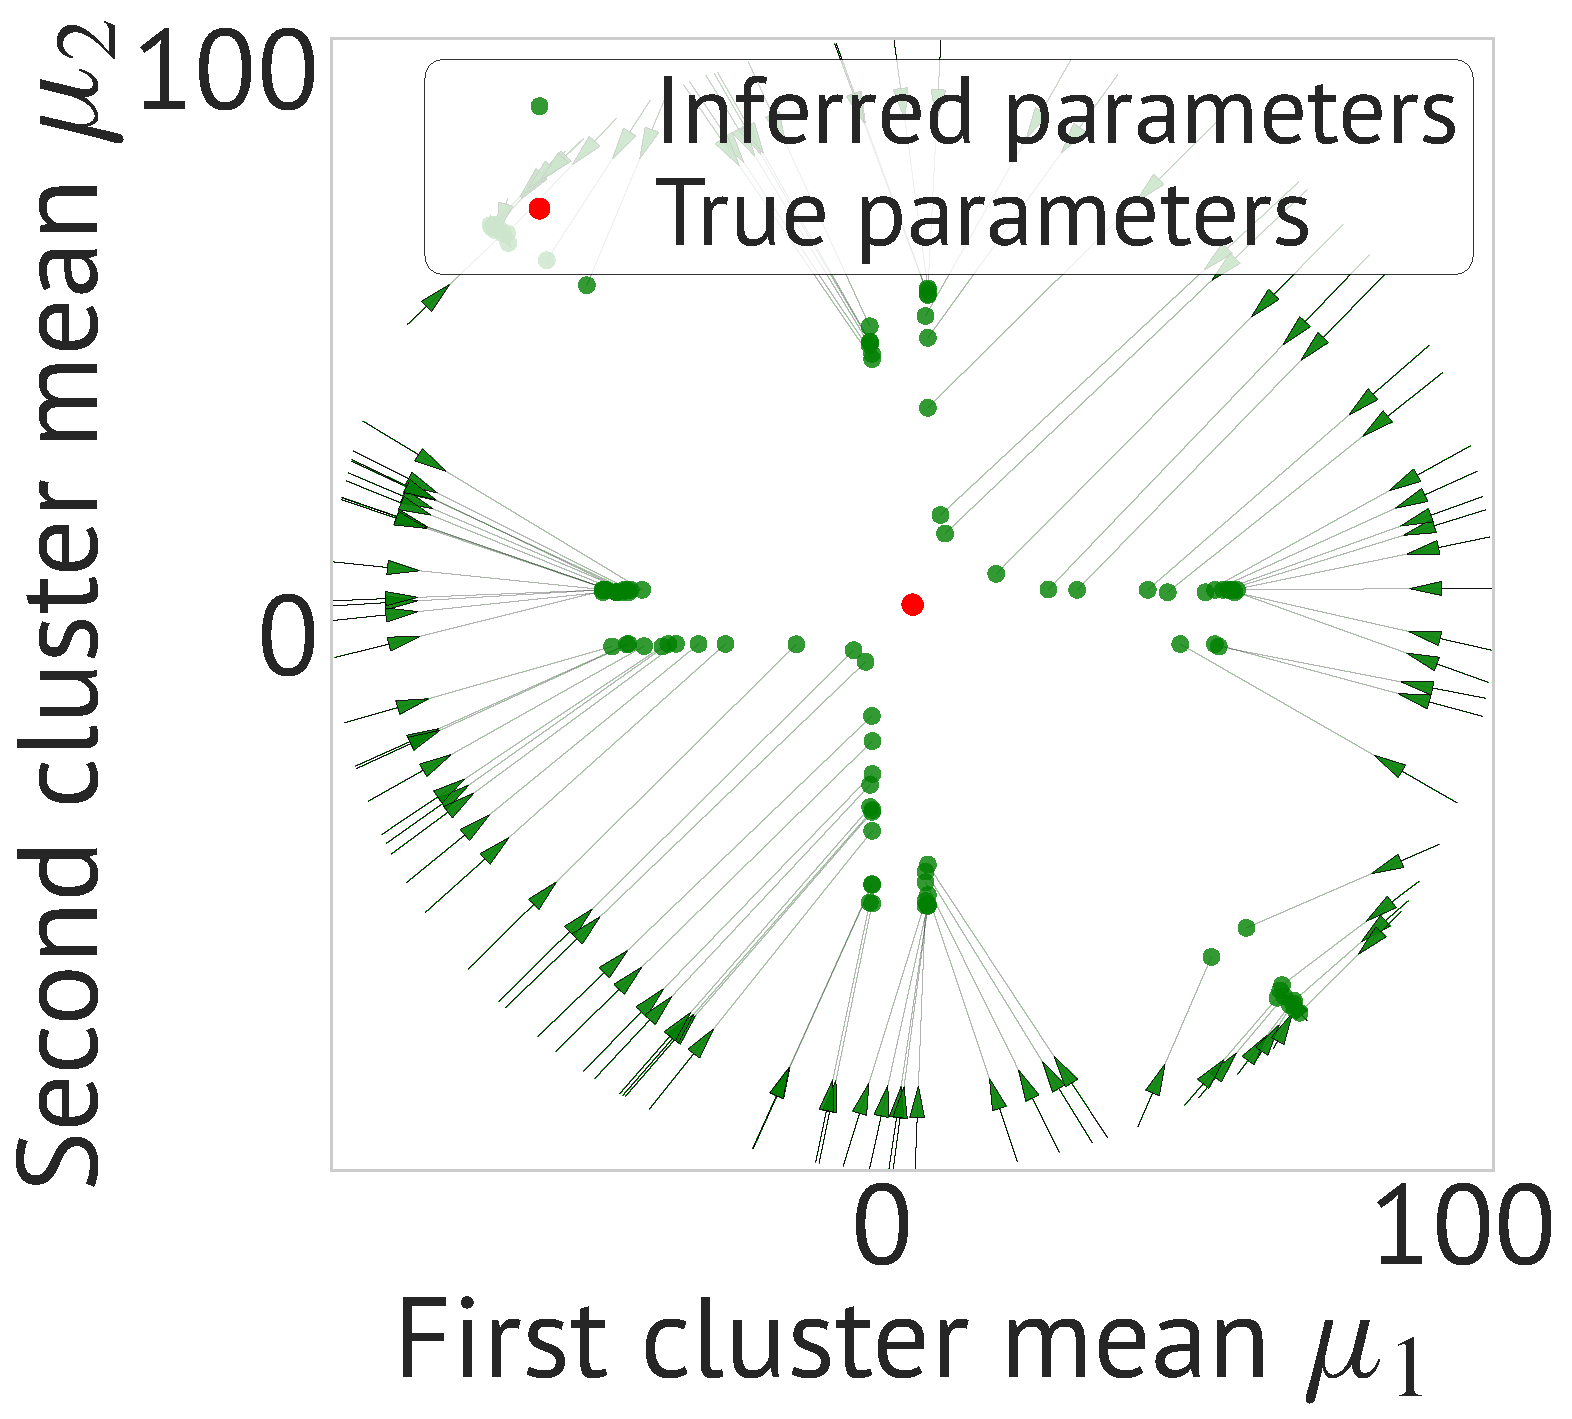
\includegraphics[width=0.8\linewidth]{ch-pvi/img/toy_vanilla}
  \label{fig:bernoulli_vanilla}
  \caption{Variational Inference}
\end{subfigure}
\begin{subfigure}{0.49\linewidth}
    \centering
    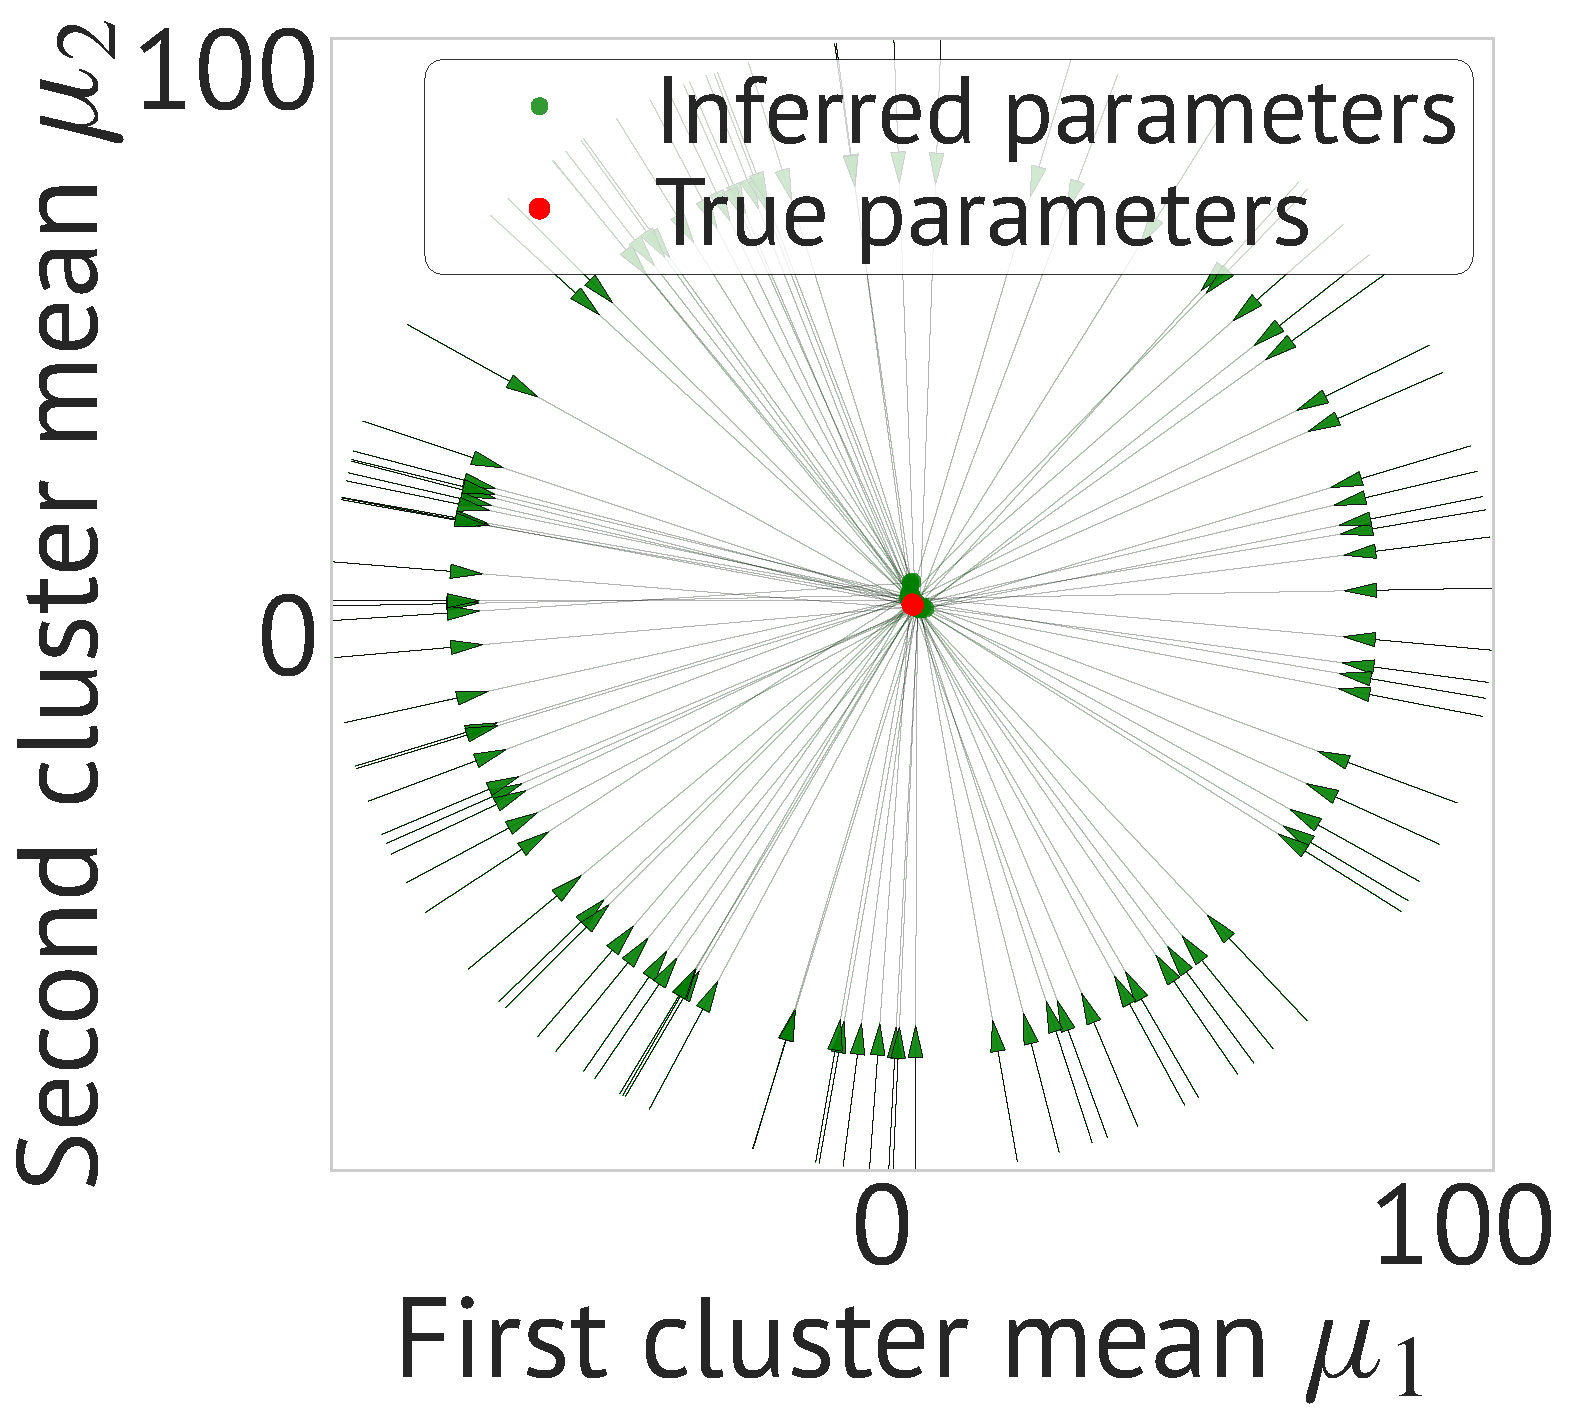
\includegraphics[width=0.8\linewidth]{ch-pvi/img/toy_global}
    \label{fig:bernoulli_global}
    \caption{Proximity \gls{vi}, \Cref{algo:global}}
\end{subfigure}
\caption[\textsc{pvi} makes \textsc{vi} robust to poor initialization]{
\textbf{\Acrlong{PVI} is robust to bad initialization.} We study a Bernoulli factor model. Model parameters are randomly initialized on a ring around the known true parameters (in red) used to generate the data. The arrows start at these parameter initializations and end at the final parameter estimates (shown as green dots). \textbf{(a)} Variational inference with gradient ascent suffers from multiple local optima and cannot reliably recover the truth. \textbf{(b)} \gls{PVI} with an entropy proximity statistic reliably infers the true parameters using \Cref{algo:global}.
}
\label{fig:bernoulli_arrows}
\end{figure*}
The issues around \gls{VI} stem from the \gls{ELBO} and the iterative algorithms used to optimize it. When the algorithm zeroes (or nearly zeroes) some of the support of $q(\mbz ; \mblambda)$, it becomes hard to later ``escape,'' i.e., to add support for the configurations of the latent variables that have been assigned zero probability~\citep{mackay2003information, Burda2016}. This leads to poor local optima and to sensitivity to the starting point, where a misguided initialization will lead to such optima. These problems happen in both gradient-based and coordinate ascent methods. We address these issues with \glsreset{PVI} \gls{PVI}, a variational inference algorithm that is specifically designed to avoid poor local optima and to be robust to different initializations.

\gls{PVI} builds on the proximity perspective of gradient ascent.  The proximity perspective views each step of gradient ascent as a constrained minimization of a Taylor expansion of the objective around the previous step's parameter~\citep{Spall:2003,boyd2004convex}.  The constraint, a \textit{proximity constraint}, enforces that the next point should be inside a Euclidean ball of the previous.  The step size relates to the size of that ball. We construct \gls{PVI} by questioning whether such a Euclidan distance-based constraint is appropriate, and whether other notions of proximity may be useful in constraining gradient ascent steps.

In \gls{VI}, a constraint on the Euclidean distance means that all dimensions of the variational parameters are equally constrained. We posit that this leads to problems; some dimensions need more regularization than others. For example, consider a variational distribution that is Gaussian.  A good optimization will change the variance parameter more slowly than the mean parameter to prevent rapid changes to the support.  The Euclidean constraint cannot enforce this. Furthermore, the constraints enforced by gradient descent are transient; the constraints are relative to the previous iterate---one poor move during the optimization can lead to permanent optimization problems.

To this end, \gls{PVI} uses proximity constraints that are more meaningful to variational inference and to optimization of probability parameters.  A constraint is defined using a proximity statistic and distance function. As one example, we consider a constraint based on the entropy proximity statistic. This limits the change in entropy of the variational approximation from one step to the next.  Consider again a Gaussian approximation. The entropy is a function of the variance alone and thus the entropy constraint counters the pathologies induced by the Euclidean proximity constraint. We also study constraints built from other proximity statistics, such as those that penalize the rapid changes in the mean and variance of the approximate posterior.

\Cref{fig:bernoulli_arrows} provides an illustration of the advantages of \gls{PVI}.  Our goal is to estimate the parameters of a factor analysis model with variational inference, i.e., using the posterior expectation under a fitted variational distribution.  We run variational inference $100$ times, each time initializing the estimates (the model parameters) to a different position on a ring around the truth.

In the figure, red points indicate the true value. The start locations of the green arrows indicate the initialized estimates. Green points indicate the final estimates, after optimizing from the initial points. Panel (a) shows that optimizing the standard \gls{ELBO} with gradients leads to poor local optima and misplaced estimates.  Panel (b) illustrates that regardless of the initialization, \gls{PVI} with an entropy proximity statistic finds estimates that are close to the true value.

The rest of this chapter is organized as follows. \Cref{sec:variational_inference} reviews variational inference and the proximity perspective of gradient optimization.  \Cref{sec:pvi} derives \gls{PVI}; we develop four proximity constraints and two algorithms for optimizing the \gls{ELBO}. We study four models in \Cref{sec:pvi-experiments}: a Bernoulli factor model, a sigmoid belief network \citep{Mnih:2016:VIM:3045390.3045621}, a variational autoencoder~\citep{kingma2014autoencoding,rezende2014stochastic}, and a deep exponential family model of text~\citep{ranganath2015deep}. \gls{PVI} outperforms classical methods for variational inference.

% !TEX root = ../main.tex
\parhead{Related Work.}  Recent work has proposed several related algorithms. \citet{khan2015kullback} and \citet{Theis2015} develop a method to optimize the \gls{ELBO} that imposes a soft limit on the change in \gls{KL} of consecutive variational approximations. This is equivalent to \gls{PVI} with identity proximity statistics and a \gls{KL} distance function. \citet{Khan:2016:FSV:3020948.3020982} extend both prior works to other divergence functions. Their general approach is equivalent to \gls{PVI} identity proximity statistics and distance functions given by strongly-convex divergences. Compared to prior work, \gls{PVI} generalizes to a broader class of proximity statistics. We develop proximity statistics based on entropy, \gls{KL}, orthogonal weight matrices, and the mean and variance of the variational approximation.

The problem of model pruning in variational inference has also been studied and
analytically solved in a matrix factorization model in \citet{nakajima2013}---this method is model-specific, whereas \gls{PVI} applies to a much broader class of latent variable models. Finally, deterministic annealing~\citep{Katihara:2008} consists of adding a temperature parameter to the entropy term in the \gls{ELBO} that initialized to a large value then annealed to unity during inference. This is similar to \gls{PVI} with the entropy proximity statistic which keeps the entropy stable across iterations. Deterministic annealing enforces global penalization of low-entropy configurations of latent variables rather than the smooth constraint used in \gls{PVI}, and cannot accommodate the range of proximity statistics we design in this work.
\section{Variational Inference}
\label{sec:variational_inference}

Consider a model $p(\mbx, \mbz)$, where $\mbx$ is the observed data and $\mbz$ are the latent variables.  As described in \Cref{sec:pvi-introduction}, \gls{VI} posits an approximating family $q(\mbz; \mblambda)$ and maximizes the \gls{ELBO} in \Cref{eq:ELBO}. Solving this optimization is equivalent to finding the variational approximation that minimizes \gls{KL} divergence to the exact posterior \citep{jordan1999introduction,wainwright2008graphical}.

\subsection{Gradient Ascent has Euclidean Proximity}
\label{sec:euclidean_proximity}
Gradient ascent maximizes the \gls{ELBO} by repeatedly following its gradient.  One view of this algorithm is that it repeatedly maximizes the linearized \gls{ELBO} subject to a proximity constraint on the current variational parameter~\citep{Spall:2003}. The name `proximity' comes from constraining subsequent parameters to remain close in the proximity statistic. In gradient ascent, the proximity statistic for the variational parameters is the identity function $f(\mblambda) = \mblambda $, and the distance function is the square difference.

Let $\mblambda_t$ be the variational parameters at iteration $t$ and $\rho$ be a constant. To obtain the next iterate $\mblambda_{t+1}$, gradient ascent maximizes the linearized \gls{ELBO},
\begin{align}
  \label{eq:linearized-elbo}
  % \begin{split}
    U(\mblambda_{t+1}) = %&
    \cL(\mblambda_t) +
    \nabla\cL(\mblambda_t)^\top(\mblambda_{t+1}-\mblambda_t) %\\
     - %&
    \frac{1}{2\rho} (\mblambda_{t+1}-\mblambda_t)^\top
    (\mblambda_{t+1}-\mblambda_t).
  % \end{split}
\end{align}
Specifically, this is the linearized \gls{ELBO} around $\mblambda_t$, subject to $\mblambda_{t+1}$ being close to $\mblambda_t$ in squared Euclidean distance.

Finding the $\mblambda_{t+1}$ which maximizes \Cref{eq:linearized-elbo} yields
\begin{align}
  \mblambda_{t+1} = \mblambda_t + \rho
  \nabla\cL(\mblambda_t). \label{eq:standard_update}
\end{align}
This is the familiar gradient ascent update with a step size of $\rho$. The step size $\rho$ controls the radius of the Euclidean ball which demarcates valid next steps for the parameters.  Note that the Euclidean constraint between subsequent iterates is implicit in all gradient ascent algorithms.

\subsection{An Example where Variational Inference Fails}
\label{sec:bernoulli_factor_model}
We study a setting where variational inference suffers from poor local optima. Consider a factor model, with Bernoulli latent variables and Gaussian likelihood:
\begin{align}
z_{ik}~&\sim~\textrm{Bernoulli}(\pi) \\
x_i~&\sim~\textrm{Gaussian}\left(\mu = \textstyle \sum_k z_{ik}
        \mu_k, \sigma^2=1\right).
\end{align}
This is a ``feature'' model of real-valued data $x$; when one of the features is on (i.e., $z_{ik}=1$), the $i$th mean shifts according the that feature's mean parameter (i.e., $\mu_{k}$).  Thus the binary latent variables $z_{ik}$ control which cluster means $\mu_k$ contribute to the distribution of $x_i$.

The Bernoulli prior is parametrized by $\pi$; we choose a Bernoulli approximate posterior $q(z_k;\lambda_k)~=~\textrm{Bernoulli}(\lambda_{k})$.  A common approach to \gls{VI} is coordinate ascent~\citep{bishop2006pattern}, where we iteratively optimize each variational parameter.  The optimal variational parameter for $z_{ik}$ is
\begin{align}
  \label{eq:z_update} \lambda_{ik} \propto
   \exp \left\{\E_{-z_{ik}} \left[- \frac{1}{2\sigma^2}(x_i -
    \sum_{j} z_{ij} \mu_j)^2\right]\right\}.
\end{align}
We can use this update in a variational expectation-maximization setting.  The
corresponding gradient for $\mu_k$ is
\begin{align}
  \label{eq:mu-gradient}
  \frac{\partial \cL}{\partial\mu_k}
  &= -
    \frac{1}{\sigma^2}\sum_i
    \left(-x_i \lambda_{ik} + \lambda_{ik} \mu_k
    + \lambda_{ik} \sum_{j \neq k}\lambda_{ij}\mu_j\right).
\end{align}
Meditating on these two equations reveals a deficiency in mean field variational inference.  First, if the mean parameters $\mu$ are initialized far from the data then $q^*(z_{ik} = 1)$ will be very small.  The reason is in \Cref{eq:z_update}, where the squared difference between the data $x_i$ and the expected cluster mean will be large and negative.  Second, when the probability of cluster assignment is close to zero, $\lambda_{ik}$ is small.  This means that the norm of the gradient in \Cref{eq:mu-gradient} will be small. Consequently, learning will be slow. We see this phenomenon in \Cref{fig:bernoulli_arrows} (a). Variational inference arrives at poor local optima and does not recover the correct cluster means.